\section{Results}\label{sec:results}

SMA-based partitioning of performance observations provides a procedural method for grouping time-correlated performance events observed during this experiment.
In the following sections, we identify regions at different timescales and apply several statistical methods over these regions to identify the breadth of performance anomalies that occur on large-scale production file systems and gain insights into their causes.

\TODO{This doesn't fit here. We have just introduced $SMA_short$ and $SMA_long$ and don't use them in this example- NJW}

\subsection{Long-term performance evolution} \label{sec:results/longterm}

The overview of performance observations in Figures \ref{fig:summary-heatmap} shows that performance degradation is often correlated in time, and these correlations can last anywhere from days to months.
Among the most striking cases of sustained performance degradation are the long periods of reduced performance for the file-per-process write workloads, depicted as dark horizontal bands, between April and August on the \cori dataset.
To characterize the extent and possible sources of these long-term abnormalities, we compare $\textup{SMA}_{short}$ to the global mean performance for each set of $J_{app, rw, sys}$ to define divergence regions where performance remained below the time-independent peak capability of the affected applications.
The resulting $\textup{SMA}_{short}$ and global mean performance for the HACC workload on \cori is shown in Figure \ref{fig:timeseries-baseline}.

Four crossovers occur between $\textup{SMA}_{short}$ and the global mean for the HACC write workload on \cori (Figure \ref{fig:timeseries-baseline}a), two of which define the extent of a long, 139-day divergence region where performance was consistently below the global mean.
The other two regions were two days and eighteen days long and were not considered relevant in the context of this long-term analysis.
In stark contrast to the HACC write workload though, the performance of HACC read workload (Figure \ref{fig:timeseries-baseline}b) was unaffected during this time.
The longest divergence region identified was 59 days long, and the median width was only four days.

These data demonstrate that the definition of an application's peak I/O performance can vary over the service life of a storage system and its dependent components.
Furthermore, the difference between the read and write motifs in Figure \ref{fig:timeseries-baseline} indicates that not all workloads are affected by long-term variation equally. 
In this case of HACC on \cori, write performance was adversely impacted for a period of months while read performance of the same I/O pattern was completely unaffected.

In combination with expert knowledge, the root cause for this particular long-term performance regression was retrospectively identified using the boundaries of the 139-day divergence region.
The intersection between $\textup{SMA}_{short}$ and the global mean in Figure \ref{fig:timeseries-baseline} occurred on March 24 and August 10.
Comparing these dates to the service history of \cori revealed that operating system upgrades occurred on exactly those dates--March 24 and August 10.
The Lustre versions were updated on those two dates, and the appearance and subsequent disappearance of the anomalous behavior was attributed to a bug in the Lustre software.
% March 24 was the upgrade of CLE6UP01 to UP03, and August 10 was CLE6UP03 to UP04.  The performance loss in t > Aug 10 is caused by Lustre bug LU-9574
%\TODO{Has this bug affected IOR/fpp R/W the same way? That could confirm (to some extent) that all apps with similar I/O patterns might have suffered from this bug. Has this bug affected shared file patterns similarly? -- Suren
%\\
%Glenn: Yes, Figure \ref{fig:regions-heatmap}b shows that ior/fpp/write was also affected, but none of the other benchmarks were.}







\subsection{Detection and attribution of transitions between divergence regions} \label{sec:results/transitions}

\begin{figure}
    \centering
    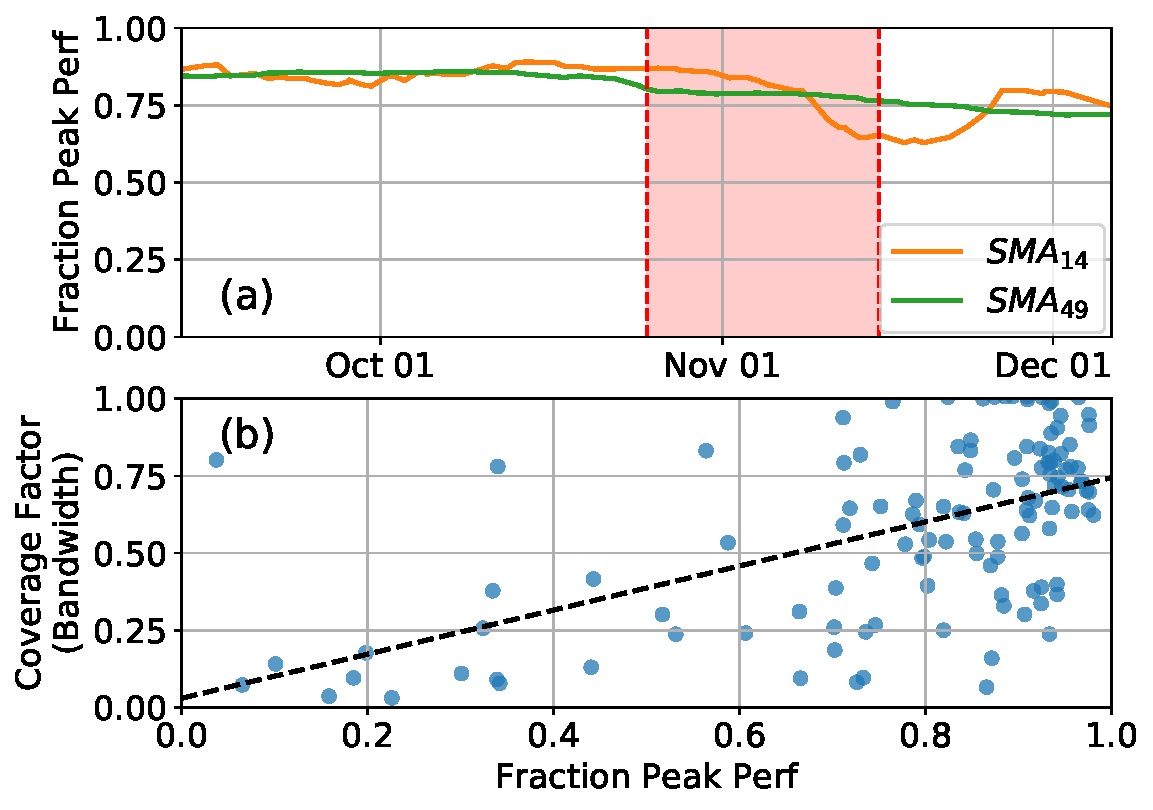
\includegraphics[width=1.0\columnwidth]{mira-correlation-region}
    \vspace{-.35in}
    \caption{Correlation between performance and $CF_{bw}$ in a transition between divergence regions on \mira for all I/O motifs combined.
    (a) shows a region automatically detected using the centroid method, and (b) shows the correlation between performance and $CF_{bw}$ in that region.
    Correlation coefficient is $0.565$ and p-value is ${1.48 \times 10^{-11}}$; dashed line in (b) is a linear fit with slope $0.714$ drawn for visual aid.}
    \label{fig:mira-correlation-region}
    % source: sc18_centroids-for-paper.ipynb
\end{figure}

%Long-term behavior has very low frequency by definition, so analyzing the causes of a few long-term performance depressions by hand (as was done in Section \ref{sec:results/longterm}) is not unreasonable.
%With smaller values of $w_{long}$, though, this method identifies an increasing number of divergence regions, and characterizing the factors that contribute to these long-term performance depressions using automated statistical techniques becomes imperative.

In order to detect and explain changes in measured performance, we need to correlate the measured performance with the other telemetric data described in Section~\ref{sec:methods}. To begin this analysis we convert pairs of divergence regions into \emph{trend regions} as described in Section \ref{sec:features}. We then perform statistical analysis across these trend regions to enable determination of the reasons for performance changes. 

%We then discard divergence regions whose $\textup{SMA}_{short}$ exhibit minimal change between their first and last value in the region.  For each divergence region bounded by times $t_0$ and $t_f$, we then discard those regions where
%
%\begin{equation}
%abs \left (
%\frac
%	{ \textup{SMA}_{short}(t_0) - \textup{SMA}_{short}(t_f) }
%	{\textup{SMA}_{short}(t_f)}
%\right ) < C
%\end{equation}
%
%and $C$ is a cutoff threshold typically between 0.15 and 0.40 whose optimal value is a function of $w_{short}$, $w_{long}$, and how variable the storage system performance tends to be over long periods of time.
%Given a well-chosen $C$, the result set of divergence regions satisfy both the (\ref{sec:results/transitions/criterion1}) sampling criterion and (\ref{sec:results/transitions/criterion2}) diversity criterion.

To demonstrate the utility of this approach, we apply it to the entirety of performance observations across all benchmarks run on \mira.
Our analysis identifies eleven divergence regions across the entire year, and for each of the corresponding trend regions, we then calculate the Pearson correlation coefficient between the fraction peak performance observations and the other telemetric data associated with each job as described in Section \ref{sec:methods/tokio}.

\TODO{These 11 were across all benchmarks ? Read and Write equally ?- NJW}

Discarding all correlations except those with extremely high confidence ($\textup{p-value} > {1.0 \times 10^{-5}}$), only five of the eleven regions exhibited moderate correlation ($R > 0.35$) between performance and any other metric.
Furthermore, the bandwidth coverage factor was the sole metric that showed compelling correlation with performance in these five regions, with correlation coefficients ranging from +0.399 to +0.590. 

An example of one of these regions and the correlation between performance and bandwidth coverage factor observed within is shown in Figure \ref{fig:mira-correlation-region}.
During this region, $\textup{SMA}_{short}$ fell from a 0.868 fraction of peak performance to 0.654 over 21 days, representing a significant loss of performance.
While this correlative analysis does not prove the cause of this event, this analysis confidently identified a long-term performance transition between October 25 and November 15 that was strongly correlated ($R = 0.565$) with bandwidth contention.
Additionally, this correlation with performance degradation was observed across \emph{all} I/O motifs (similar to Figure \ref{fig:regions-heatmap}a) distinguishes it from the case discussed in section \ref{sec:results/longterm} and further indicates a system-wide loss of performance.
The relative rarity of an event of this magnitude on \mira further suggests that the contentious activity coincident with this performance depression on \mira was likely not caused by routine job traffic and may have been related to year-end activity on the system.

\begin{figure}
    \centering
    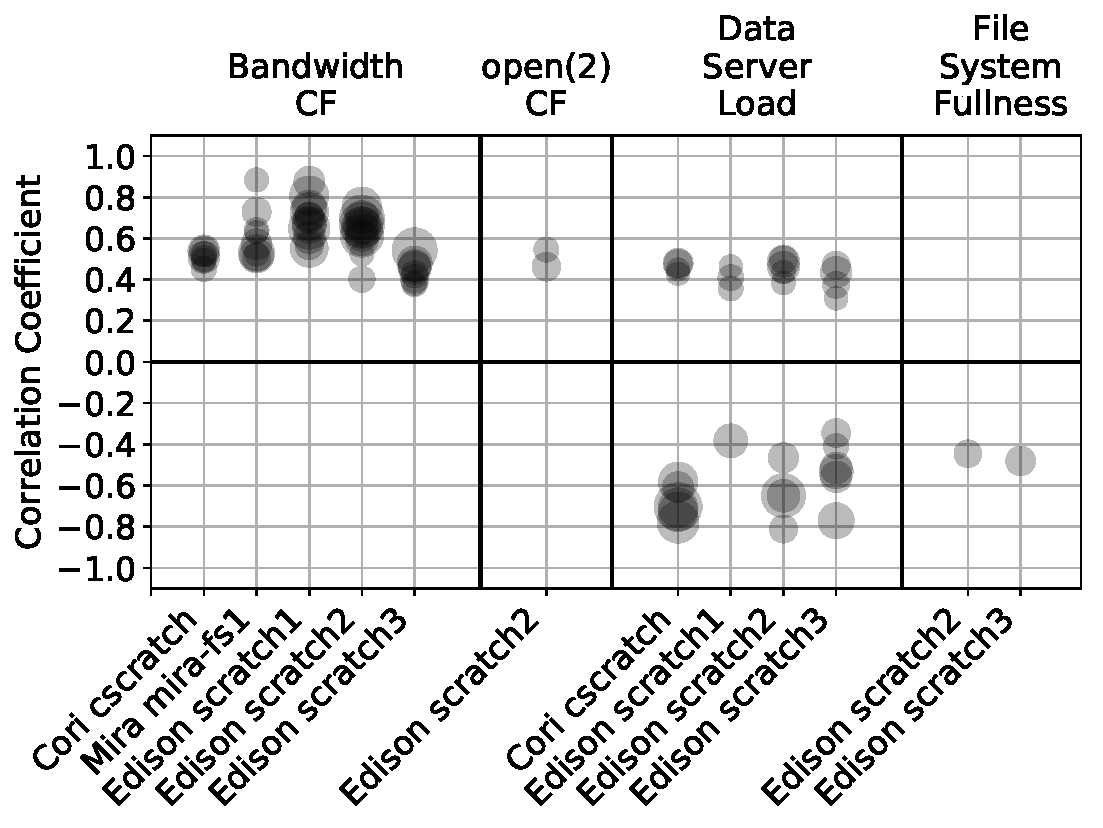
\includegraphics[width=1.0\columnwidth]{trend-correlations}
    \vspace{-.35in}
    \caption{Correlations discovered between fraction peak performance and all other metrics measured during job execution.
    Each circle represents the correlation coefficient over a single trend region, and its diameter is proportional to $-\log_{10}(\textup{p-value}$).
    CF denotes coverage factor.}
    \label{fig:trend-correlations}
    % source: sc18_centroids-allsystems.ipynb
\end{figure}


\begin{figure}
    \centering
    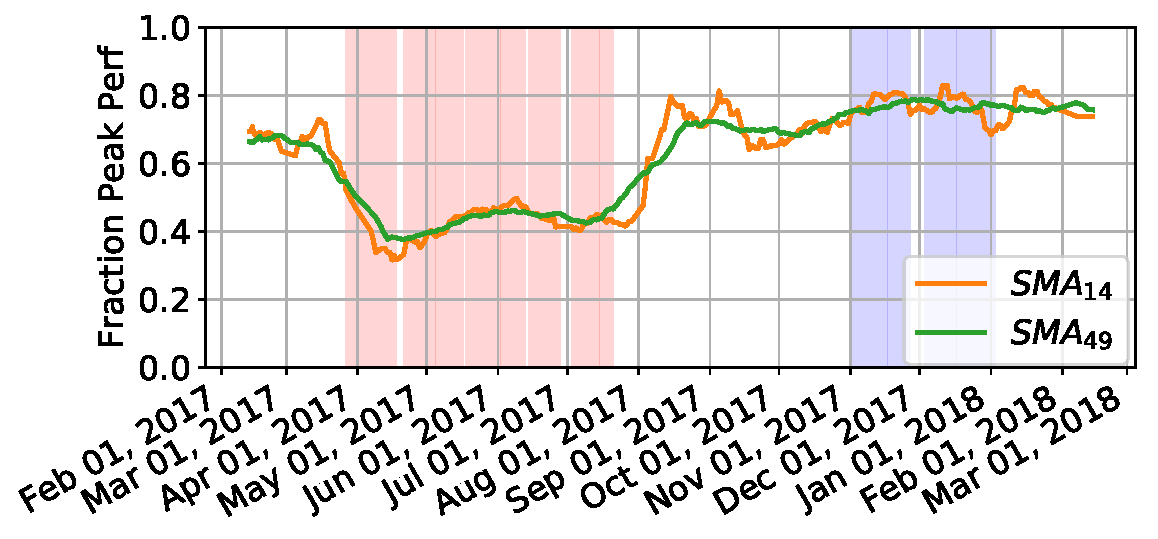
\includegraphics[width=1.0\columnwidth]{cscratch-bimodal-fsaveosscpu}
    \vspace{-.35in}
    \caption{Regions of negative correlation (red) and positive correlation (blue) between fraction peak performance and data server load during trend regions identified on \cori.
    SMAs for \cori's HACC write workload also shown to illustrate the coincidence of a long-term performance issue with the direction of correlation.}
    \label{fig:cscratch-bimodal-fsaveosscpu}
    % source: sc18_centroids-allsystems.ipynb
\end{figure}

%The results found in Figure \ref{fig:mira-correlation-region} are only governed by a single input parameter (the maximum p-value to show), it can be trivially extended to all other storage systems tested in this study with no additional parametric tuning.
%Doing so results in a set of trend regions where performance was found to correlate moderately with other measured parameters as the performance evolved, providing a more holistic view of the factors that may contribute to these longer-term performance instabilities.

Next we apply the same correlation analysis to the other machines in our study, again only keeping correlations with an extremely high confidence ($\textup{p-value} > {1.0 \times 10^{-5}}$). 
The results of this analysis are shown in Figure \ref{fig:trend-correlations}. There is Moderate correlation between performance and the bandwidth coverage factor for all the trend regions across \mira, \cori, and \edison.
Although intuitive at the scale of a single performance transient, the fact that these correlations were found over trend regions indicate that bandwidth contention from \emph{sustained workloads} often coincide with sustained performance losses.
This is particularly relevant to the increasing fraction of experimental and observational data that is being processed on modern HPC platforms; as the volume of data being continually streamed from large-scale scientific instruments increases, the effects of sustained bandwidth contention are likely to become increasingly prominent.

Another noteworthy feature that this method revealed is the bimodality of correlation between performance and the CPU load of the file system data servers ("Data Server Load" in Figure \ref{fig:trend-correlations}) on the Lustre filesystem based machines.

As shown in Figure \ref{fig:cscratch-bimodal-fsaveosscpu}, the bimodality of the correlation matches the biomodality observed in the HACC write workload on the affected storage systems.
During the long-term performance regression discussed in Section \ref{sec:results/longterm}, high CPU load on the Lustre OSSs coincided with low performance of the I/O performance probes.
As soon as performance was restored on August 10, the relationship reversed, and high CPU load was observed favorably with respect to performance.
The positive correlation between performance and CPU load is consistent with the data servers using CPUs primarily to service incoming I/O requests, whereas the negative correlation indicates that another CPU load (as may be caused by an algorithmic bug) was present and competed with the data servers' ability to use CPU to service those same requests.
Had this correlation analysis been performed without the benefit of partitioning over trend regions, the regions of positive and negative correlation would have obfuscated each other in the net result. 

\TODO{There is no text that talks about the Open CF or fullness parts of the figure here- what do you want to say?}

\subsection{Transient performance loss} \label{sec:results/shortterm}

\TODO{This is a very complicated analysis to describe completely.  Please point out places where clarification is necessary or would be helpful.}

%\begin{figure}
%    \centering
%    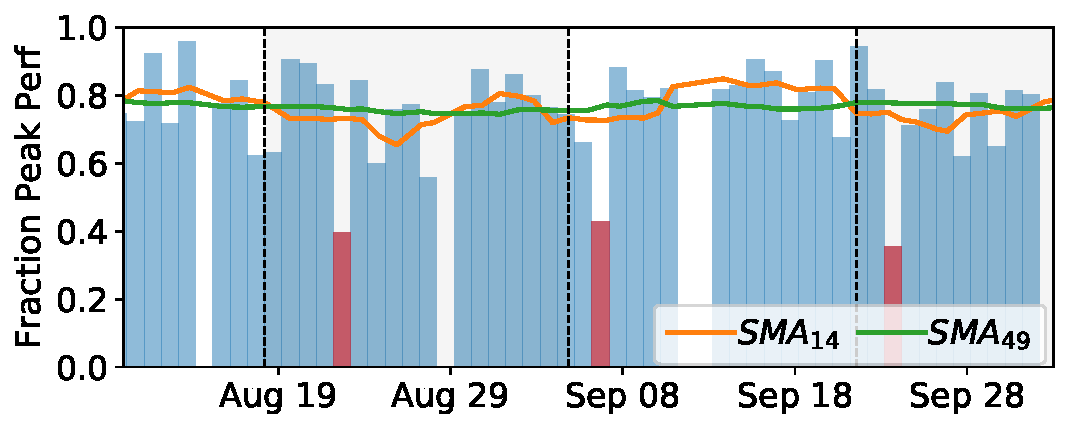
\includegraphics[width=1.0\columnwidth]{shortterm-mirafs1-dbscan}
%    \vspace{-.35in}
%    \caption{SMA partitioning and using minima in each region to identify transient.}
%    \label{fig:shortterm-mirafs1-dbscan}
%    % source: sc18_umamify.ipynb
%\end{figure}

\begin{figure}
    \centering
    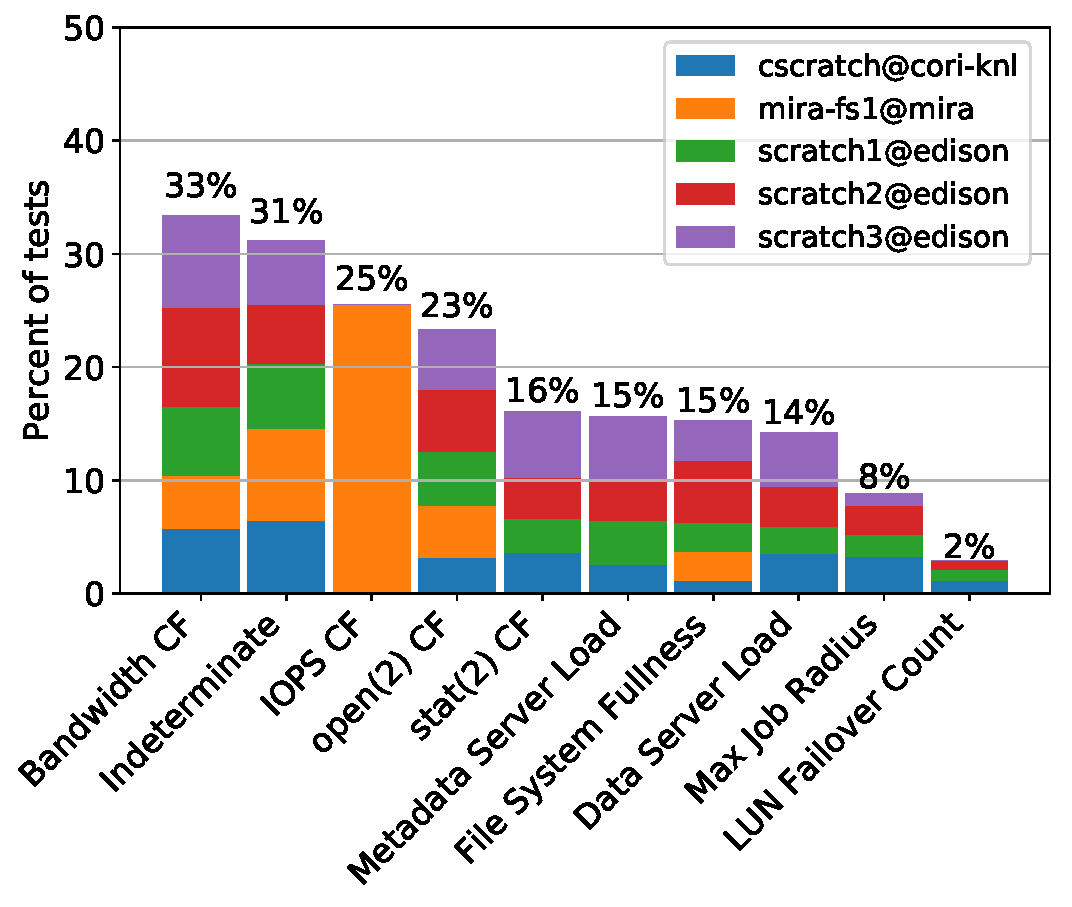
\includegraphics[width=1.0\columnwidth]{contributors-bad-by-system}
    \vspace{-.35in}
    \caption{Metrics that correlated with poor I/O performance across all file systems and benchmarks tested normalized to the number of probes during which each metric was measured.
    \mira was the only system for which IOPS coverage factor was measured. 
    These data represent 490 anomalous jobs, and 80 jobs (16\%) had no metrics classified as contributors.
    Percentages do not add up to 100\% because multiple metrics are often classified as contributors for a single anomalous job.
    }
    \label{fig:contributors-bad-by-system}
    % source: sc18_umamify-2.0.ipynb
\end{figure}

As well as being able to determine long-term performance issues it would also be advantageous to determine the reasons why I/O performance is severely degraded for one and only one day in an otherwise unremarkable period of time.
Such performance losses may only be observed in one of the I/O motifs tested on that day, suggesting a very short-lived issue that disappeared over the course of one or two of the eight daily performance probes.
The lack of a consistent performance trend surrounding these transients makes them difficult to correlate with other metrics as was done in the previous section, a different approach will be required. Understanding the contributors to these transients is critical to informing the design of storage system hardware and software as well, eventually, mitigating them. 

The performance of a particular performance result (hereafter referred to as the anomalous job) is first contextualized with respect its neighboring jobs, where neighboring jobs are those that
\begin{enumerate}[leftmargin=*]
\item ran in the same period of time, so that we comparing jobs in the same long-term divergence regions, and
\item exhibited the same I/O motif, so we are not comparing jobs whose performance variation may have resulted from having different I/O patterns
\end{enumerate}

In addition to I/O performance, telemetric data collected from other instrumentation sources throughout the I/O subsystem (as described in Section \ref{sec:methods/tokio}) are also associated with each job.
\TODO{How does this work if one jobs spans more than one time point in a telemetric series of data? - NJW}
The anomalous job is then identified as the observation with the worst performance within its divergence region, and any metrics whose worst values were also observed during the anomalous job are classified as possible contributors.
The result is zero or more metrics being flagged as potential contributors to poor performance for each divergence region, application, file system, and read/write mode. For example, if both the performance and the bandwidth coverage factor for the anomalous job are the lowest values observed amongst its neighboring jobs, we classify bandwidth coverage factor as a possible contributor to that poor performance.

%To address these transients, we apply a simple binary classification scheme where metrics are identified as either possible contributors or not.

The statistical significance of these classifications is a function of how many observations are contained in the divergence region where each positive classification is made.
For the sake of setting a limit on uncertainty, we discard all divergence regions whose classifications exceed a p-value of 0.10. \TODO{where is the p-value classification of a divergence region defined ?}
The remaining positive classifications are then grouped by metric and normalized to the number of abnormal jobs where that metric was measured.
The resulting values describe the frequency with which each metric coincides with poor performance across all of the test systems and are shown in Figure \ref{fig:contributors-bad-by-system}.

This analysis reveals that abnormally high contention for bandwidth and IOPS are the metrics that most frequently coincide with abnormally poor performance.
Contention on metadata servers and CPU load on data servers was also observed during anomalous jobs to a less significant degree, consistent with the correlation coefficients shown in Figure \ref{fig:trend-correlations}.
Unlike the correlative analysis, though these data speak directly to the conditions that are present during abnormally poor I/O performance rather than summarize conditions during longer trend periods.
Although the statistical significance of individual metric classifications is relatively high (${\textup{p-value} < 0.10}$), aggregating the classified metrics over all abnormal jobs reveals significantly greater degrees of significance.
For example, the findings shown in Figure \ref{fig:contributors-bad-by-system} all demonstrate p-values of $10^{-4}$ or lower.





\subsection {Discussion}
\label{sec:results/discussion}

\TODO{This is where interesting dribs and drabs are winding up.  Do we carve out a separate section about this stuff, or just drop it?}

Our choice of averaging $\textup{SMA}_{short}$ over ${-0.5w_{short} <= t < +0.5w_{short}}$ makes it insensitive to choice of $w_{short}$.
For the analysis in Section \ref{sec:results/longterm} changing $\textup{SMA}_{short}$ from $\textup{w}_{14}$ to both $\textup{w}_{7}$ and $\textup{w}_{28}$ resulted in no change to the dates bounding the 139-day divergence region.
The principal effect of changing $\textup{w}_{short}$ is the number of short regions that arise from the higher-frequency oscillations of $\textup{SMA}_{short}$ around $\textup{SMA}_{long}$.

\TODO{This is where a discussion about performance models having to account for long-term changes to baseline performance should go.  That doesn't seem to fit well into the rest of the narrative though.}

We found the exact choice of $w_{short}$ and $w_{long}$ to be somewhat arbitrary; adjusting these values by as much as $\pm 50\%$ did not affect the identification of the most significant events presented here.
In addition, a specific choice of $w$ does not preclude analyzing events longer or shorter than $w$, and we demonstrate methods to address this in Sections \ref{sec:results/longterm} and \ref{sec:results/shortterm}.

